
  \subsubsection{Back-end}
  \paragraph{Informazioni sul package} 
    \begin{figure}[H] 
      \begin{center} 
        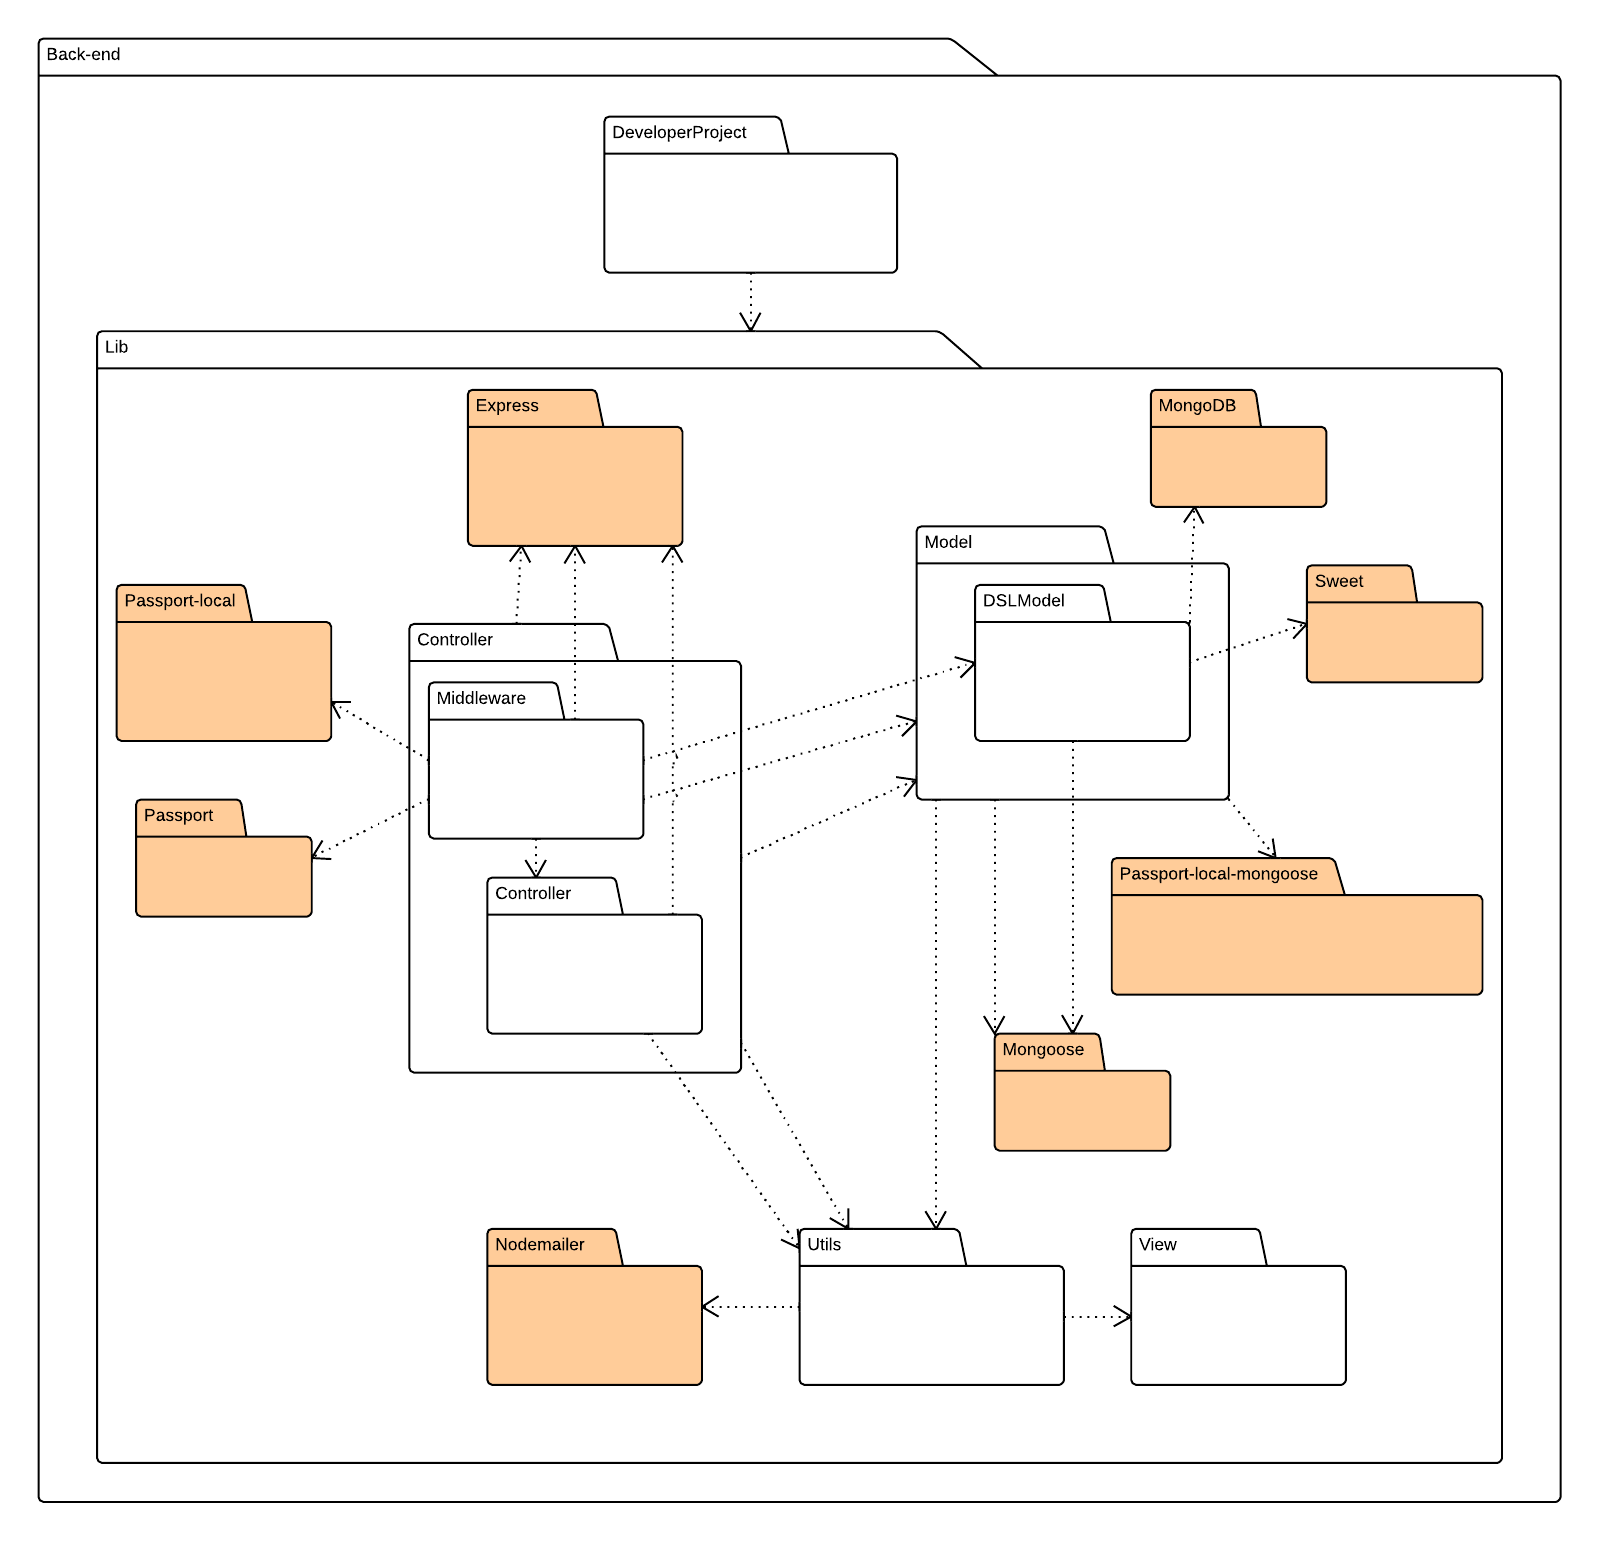
\includegraphics[width=\textwidth]{uml/package/Back-end.png}  
        \caption{Componente Back-end}
      \end{center}  
    \end{figure} 
  \subparagraph{Descrizione} 
    \begin{itemize}
    \item[] \glossario{Package} che racchiude tutta la componente di \glossario{Back-end}. Comprende la libreria dell'applicazione \textit{MaaP} e il package del progetto sviluppato dal developer che andrà ad utilizzare tale libreria.
    \end{itemize} 
    \subparagraph{Package contenuti} 
    \begin{itemize}
        \item DeveloperProject
        \item Lib
    \end{itemize}
  \subsubsection{DeveloperProject}
  \paragraph{Informazioni sul package} 
    \begin{figure}[H] 
      \begin{center} 
        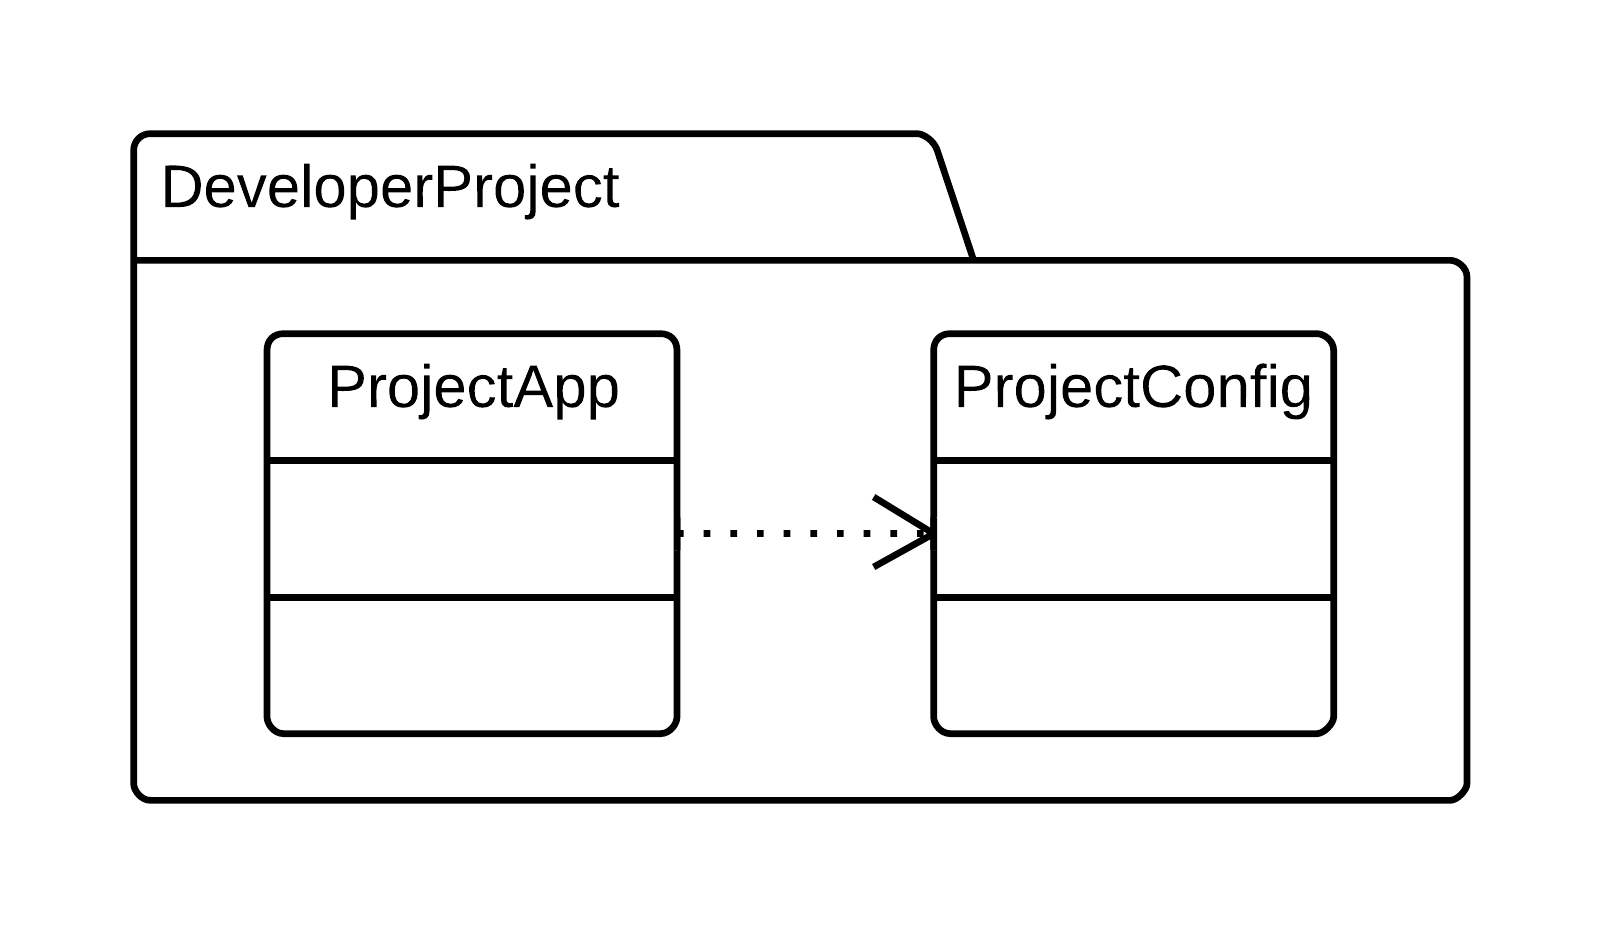
\includegraphics[width=\textwidth]{uml/package/Back-end::DeveloperProject.png}  
        \caption{Componente DeveloperProject}
      \end{center}  
    \end{figure} 
  \subparagraph{Descrizione} 
    \begin{itemize}
    \item[] Questo \glossario{Package} ha il compito di fornire la configurazione e avviare il web server di \glossario{MaaP}. Consiste negli oggetti che dovranno essere predisposti dal developer che vorrà installare il framework \glossario{MaaP}. L'installazione dell framework \glossario{MaaP} fornisce uno \glossario{scaffold} dei file e delle classi necessarie per il funzionamento dell'applicazione. Sarà compito del developer modificare tali file inserendo i dati corretti.
    \end{itemize} 
  \subparagraph{Interazioni con altri componenti} 
    \begin{itemize} 
        \item Back-end  
    \end{itemize} 
    \paragraph{Classi}
      \subparagraph{Back-end::DeveloperProject::ProjectApp}
        
        \textbf{\\ \\ Descrizione} 
          \begin{itemize}
            \item[] Classe modificabile dall'utente-developer che si occupa di configurare e avviare il server dell'applicazione.
          \end{itemize}      
        \textbf{Utilizzo}  
          \begin{itemize}
            \item[] Internamente avvia il server utilizzando la classe ServerLoader, a cui passa i parametri di configurazione del progetto definiti con un oggetto della classe ProjectConfig.
          \end{itemize}
          \textbf{Relazioni con altre classi}
          \begin{itemize}
              \item{Back-end::DeveloperProject::ProjectConfig}
              \item{Back-end::Lib::ServerLoader}
          \end{itemize}
      \subparagraph{Back-end::DeveloperProject::ProjectConfig}
        
        \textbf{\\ \\ Descrizione} 
          \begin{itemize}
            \item[] Classe che si occupa di configurare il progetto creato dallo sviluppatore.
          \end{itemize}      
        \textbf{Utilizzo}  
          \begin{itemize}
            \item[] Viene utilizzata per descrivere tutti i parametri dell'applicazione. Quando viene creata una \texttt{Back-end::Lib::ServerApp} le viene passato un oggetto di questo tipo ed essa avvierà l'applicazione a partire da questa configurazione.
          \end{itemize}
  \subsubsection{View}
  \paragraph{Informazioni sul package} 
    \begin{figure}[H] 
      \begin{center} 
        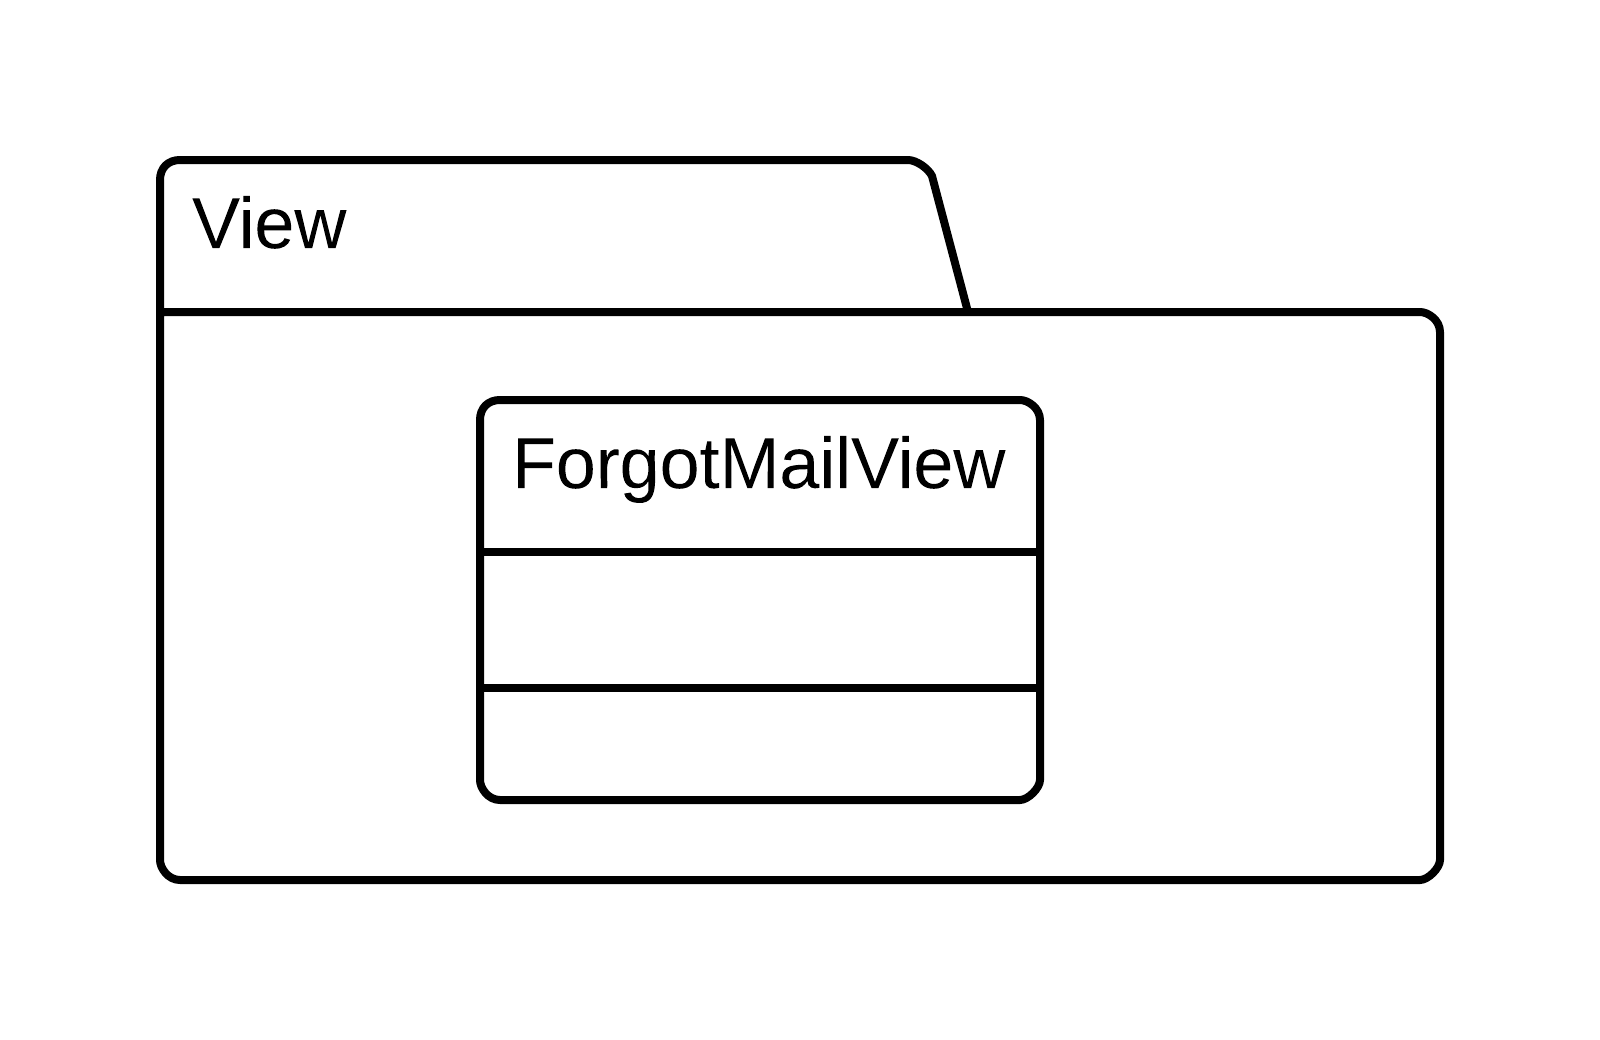
\includegraphics[width=\textwidth]{uml/package/Back-end::Lib::View.png}  
        \caption{Componente View}
      \end{center}  
    \end{figure} 
  \subparagraph{Descrizione} 
    \begin{itemize}
    \item[] \glossario{Package} contenente le classi che costituiscono i template utilizzati per le email di recupero-
password. Verranno utilizzate dal \glossario{middleware} Mailer.

    \end{itemize} 
  \subsubsection{Controller}
  \paragraph{Informazioni sul package} 
    \begin{figure}[H] 
      \begin{center} 
        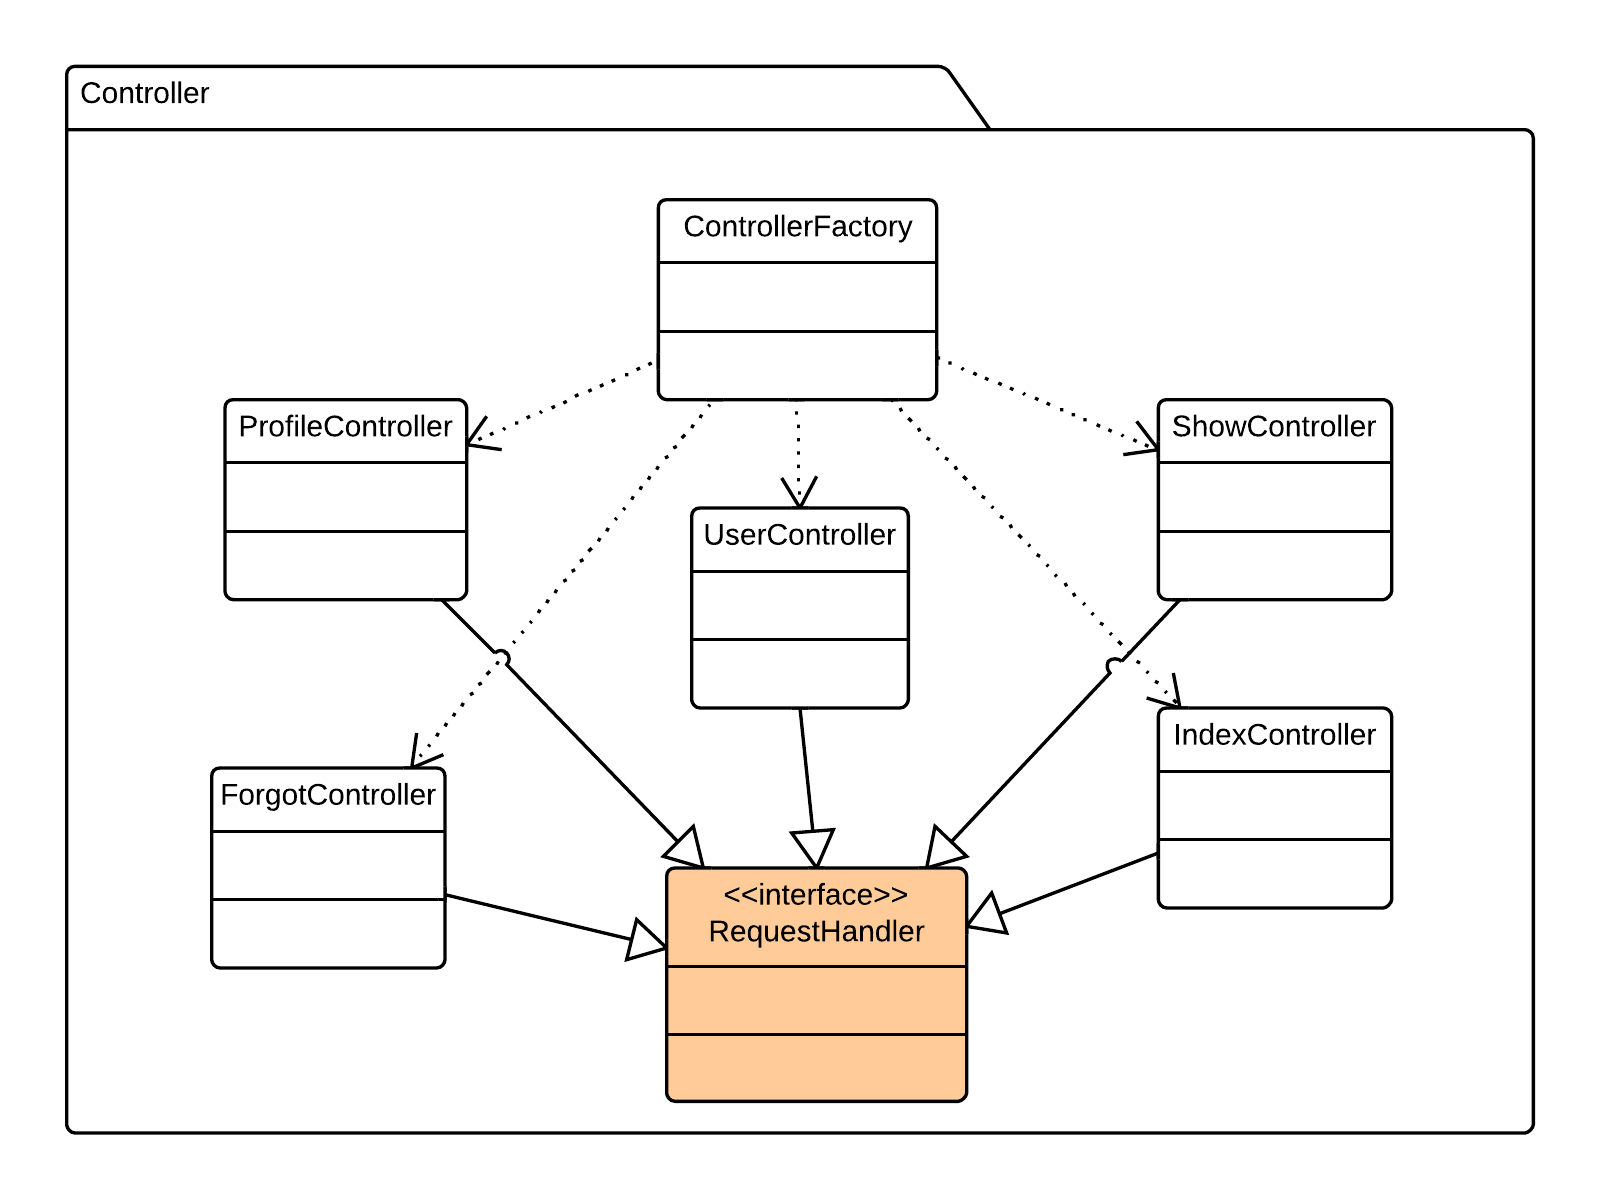
\includegraphics[width=\textwidth]{uml/package/Back-end::Lib::Controller.png}  
        \caption{Componente Controller}
      \end{center}  
    \end{figure} 
  \subparagraph{Descrizione} 
    \begin{itemize}
    \item[] 
    \end{itemize} 
    \subparagraph{Package contenuti} 
    \begin{itemize}
        \item Middleware
        \item Controller
    \end{itemize}
  \subsubsection{Model}
  \paragraph{Informazioni sul package} 
    \begin{figure}[H] 
      \begin{center} 
        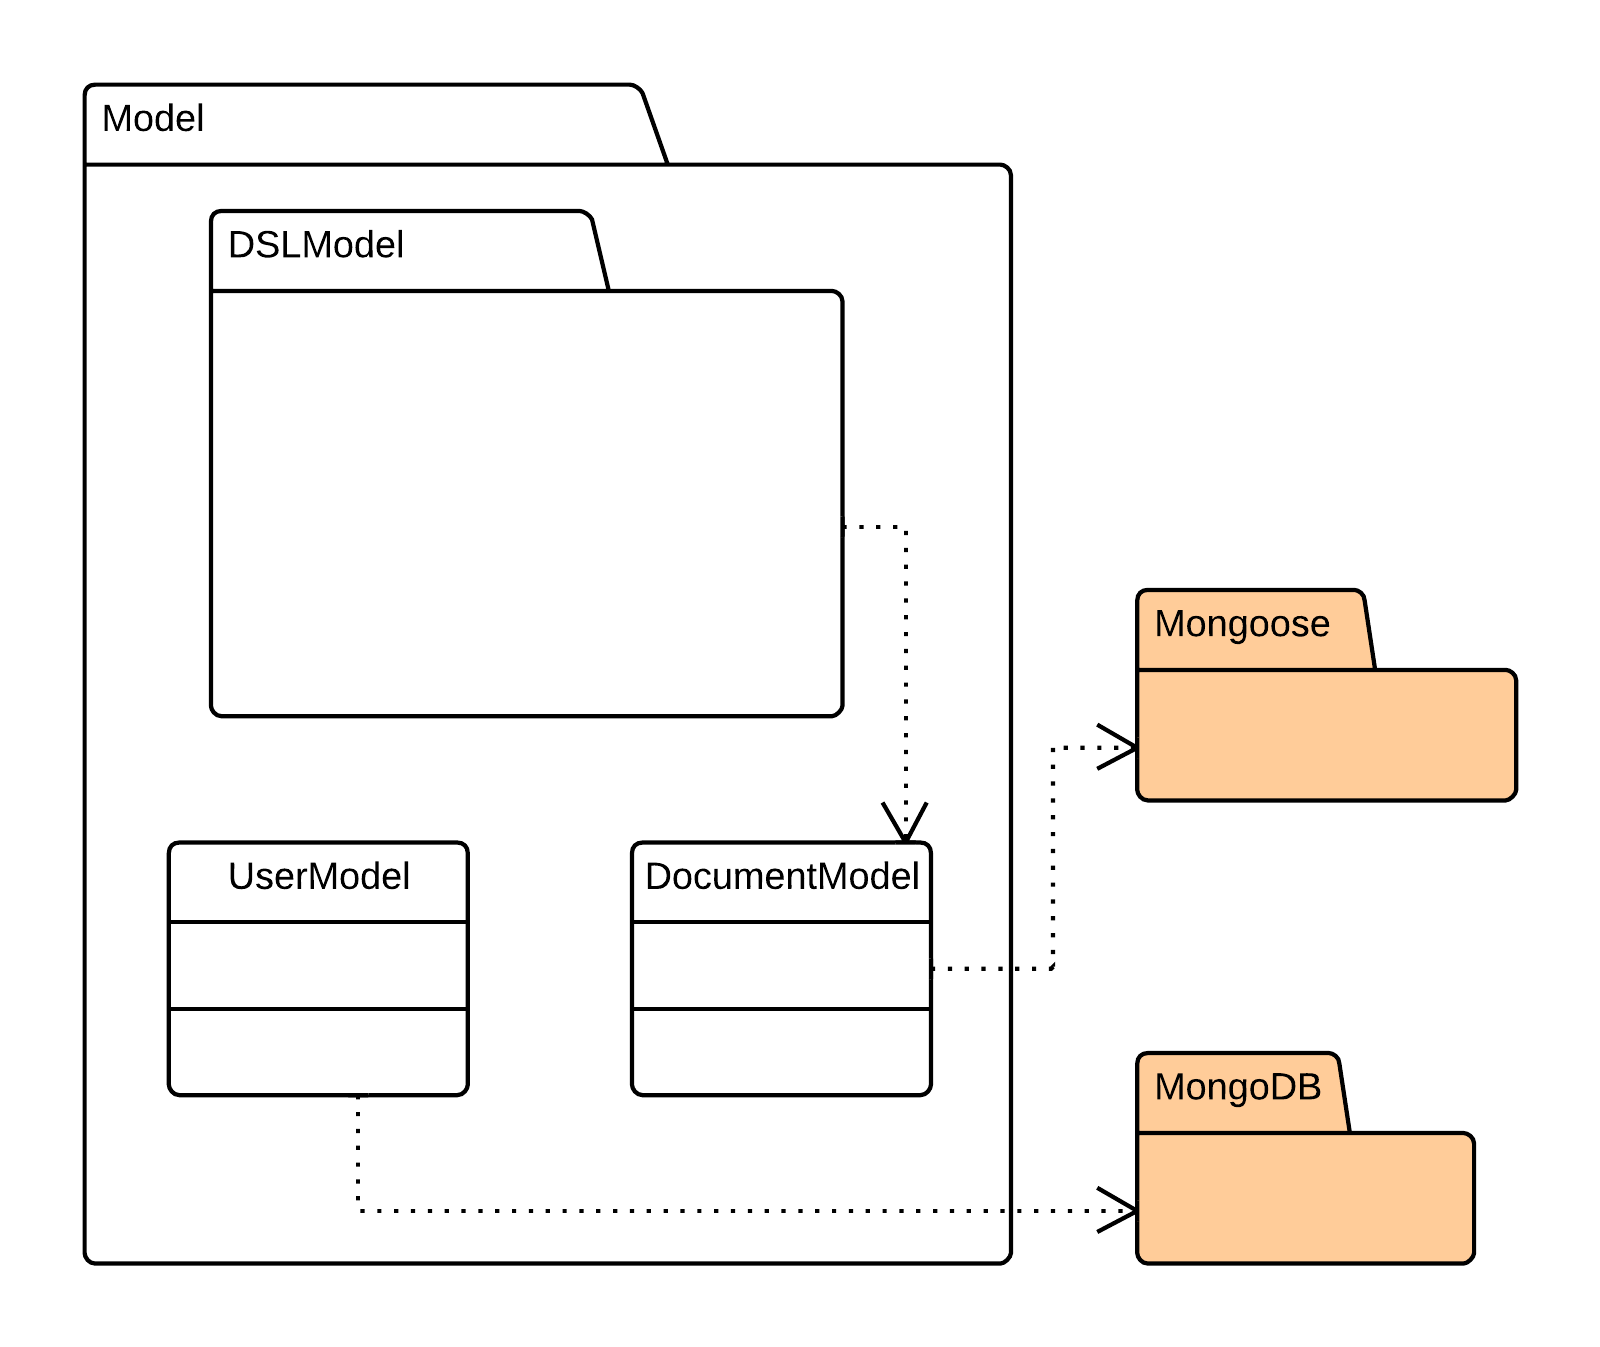
\includegraphics[width=\textwidth]{uml/package/Back-end::Lib::Model.png}  
        \caption{Componente Model}
      \end{center}  
    \end{figure} 
  \subparagraph{Descrizione} 
    \begin{itemize}
    \item[] 
    \end{itemize} 
    \subparagraph{Package contenuti} 
    \begin{itemize}
        \item DSLModel
    \end{itemize}
  \subsubsection{DSLModel}
  \paragraph{Informazioni sul package} 
    \begin{figure}[H] 
      \begin{center} 
        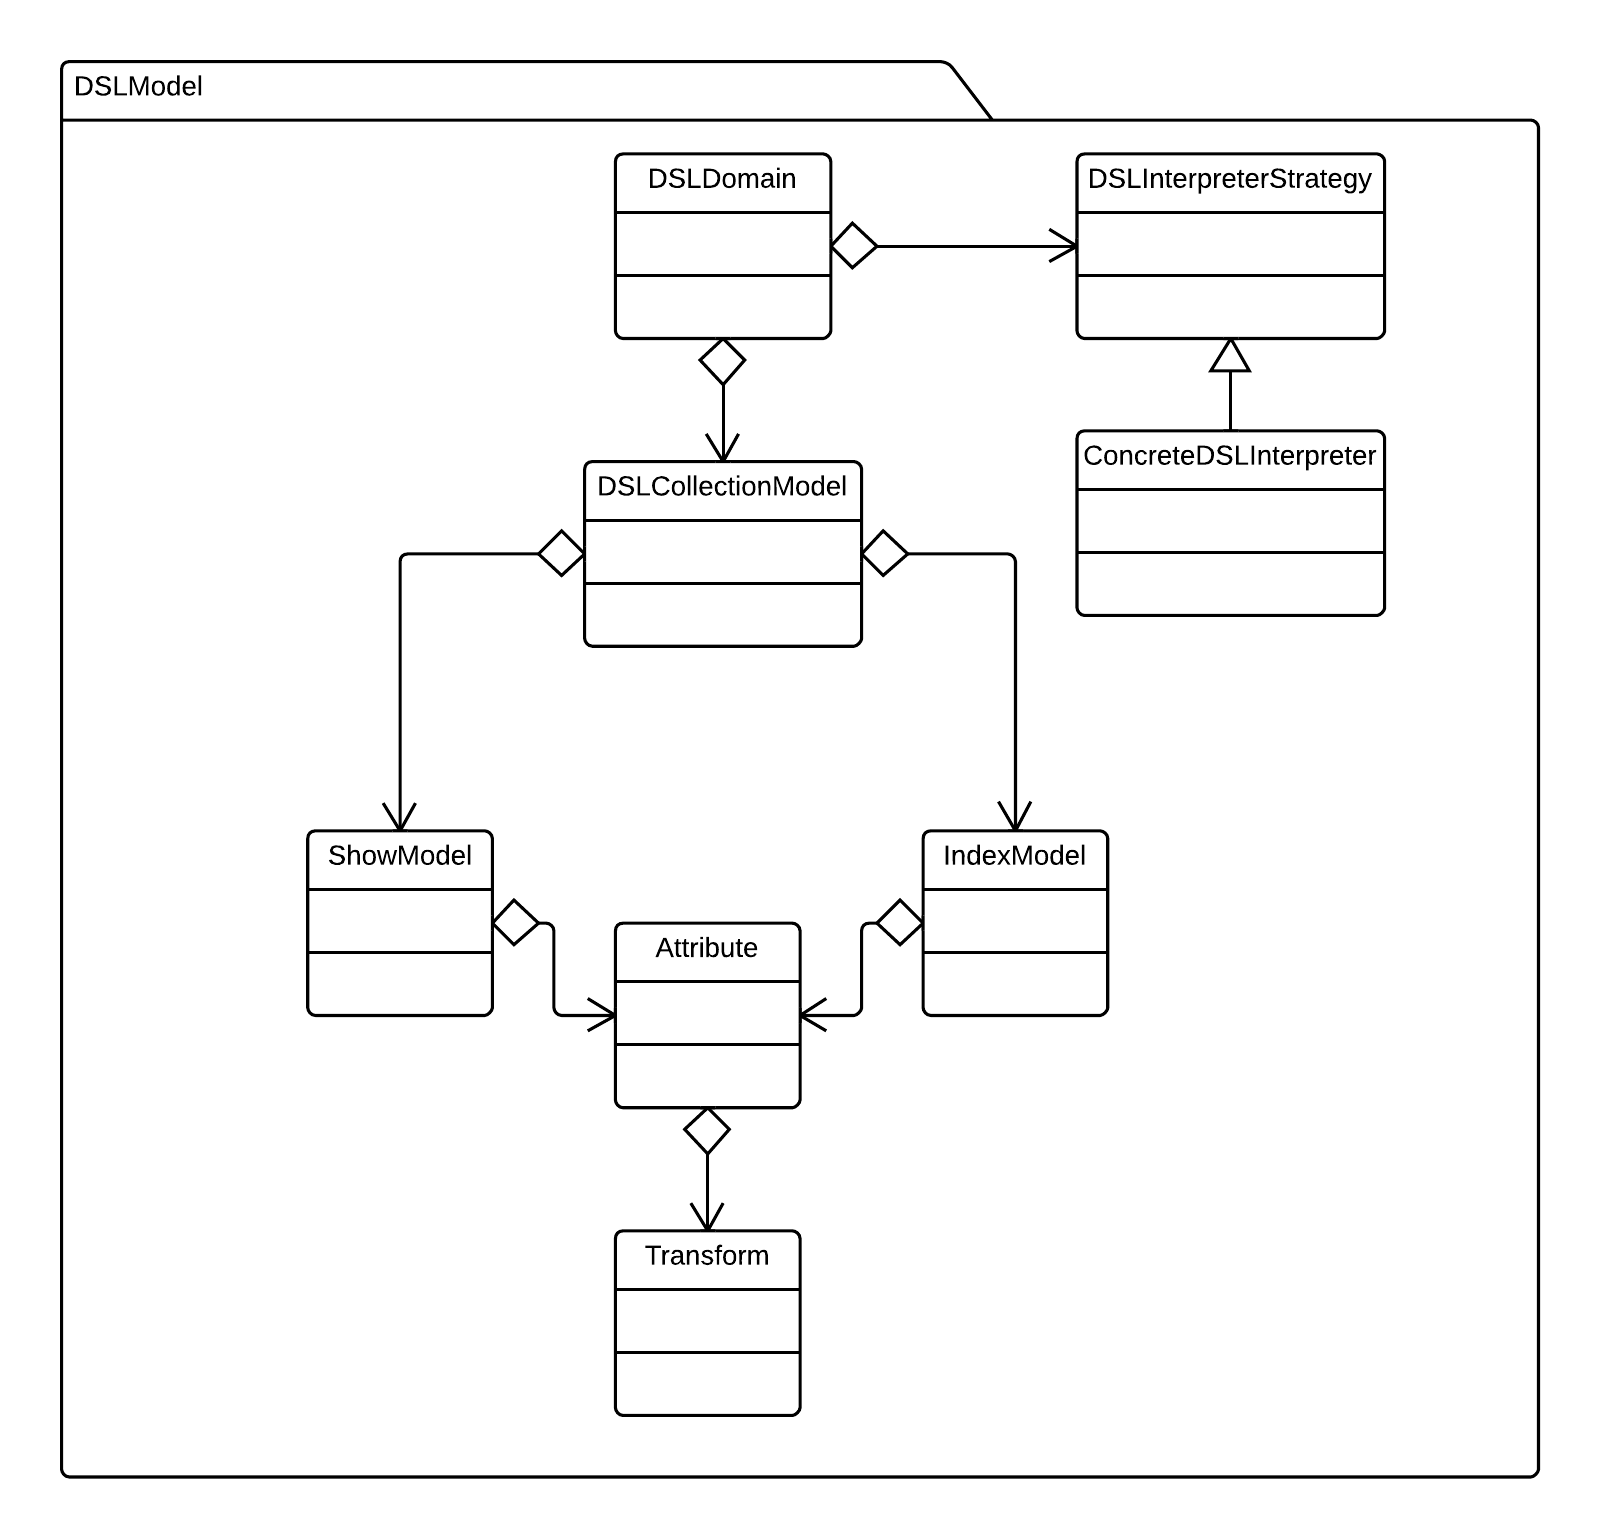
\includegraphics[width=\textwidth]{uml/package/Back-end::Lib::Model::DSLModel.png}  
        \caption{Componente DSLModel}
      \end{center}  
    \end{figure} 
  \subparagraph{Descrizione} 
    \begin{itemize}
    \item[] \glossario{Package} costituito da classi per la definizione delle regole di business sui dati definite tramite il \glossario{DSL} . Il \glossario{package} contiene principalmente classi che si occupano del caricamento del \glossario{DSL} e della sua rappresentazione in un modello ad oggetti. Costituisce la componente model dell’architettura MVC del back-end.

    \end{itemize} 
  \subsubsection{Middleware}
  \paragraph{Informazioni sul package} 
    \begin{figure}[H] 
      \begin{center} 
        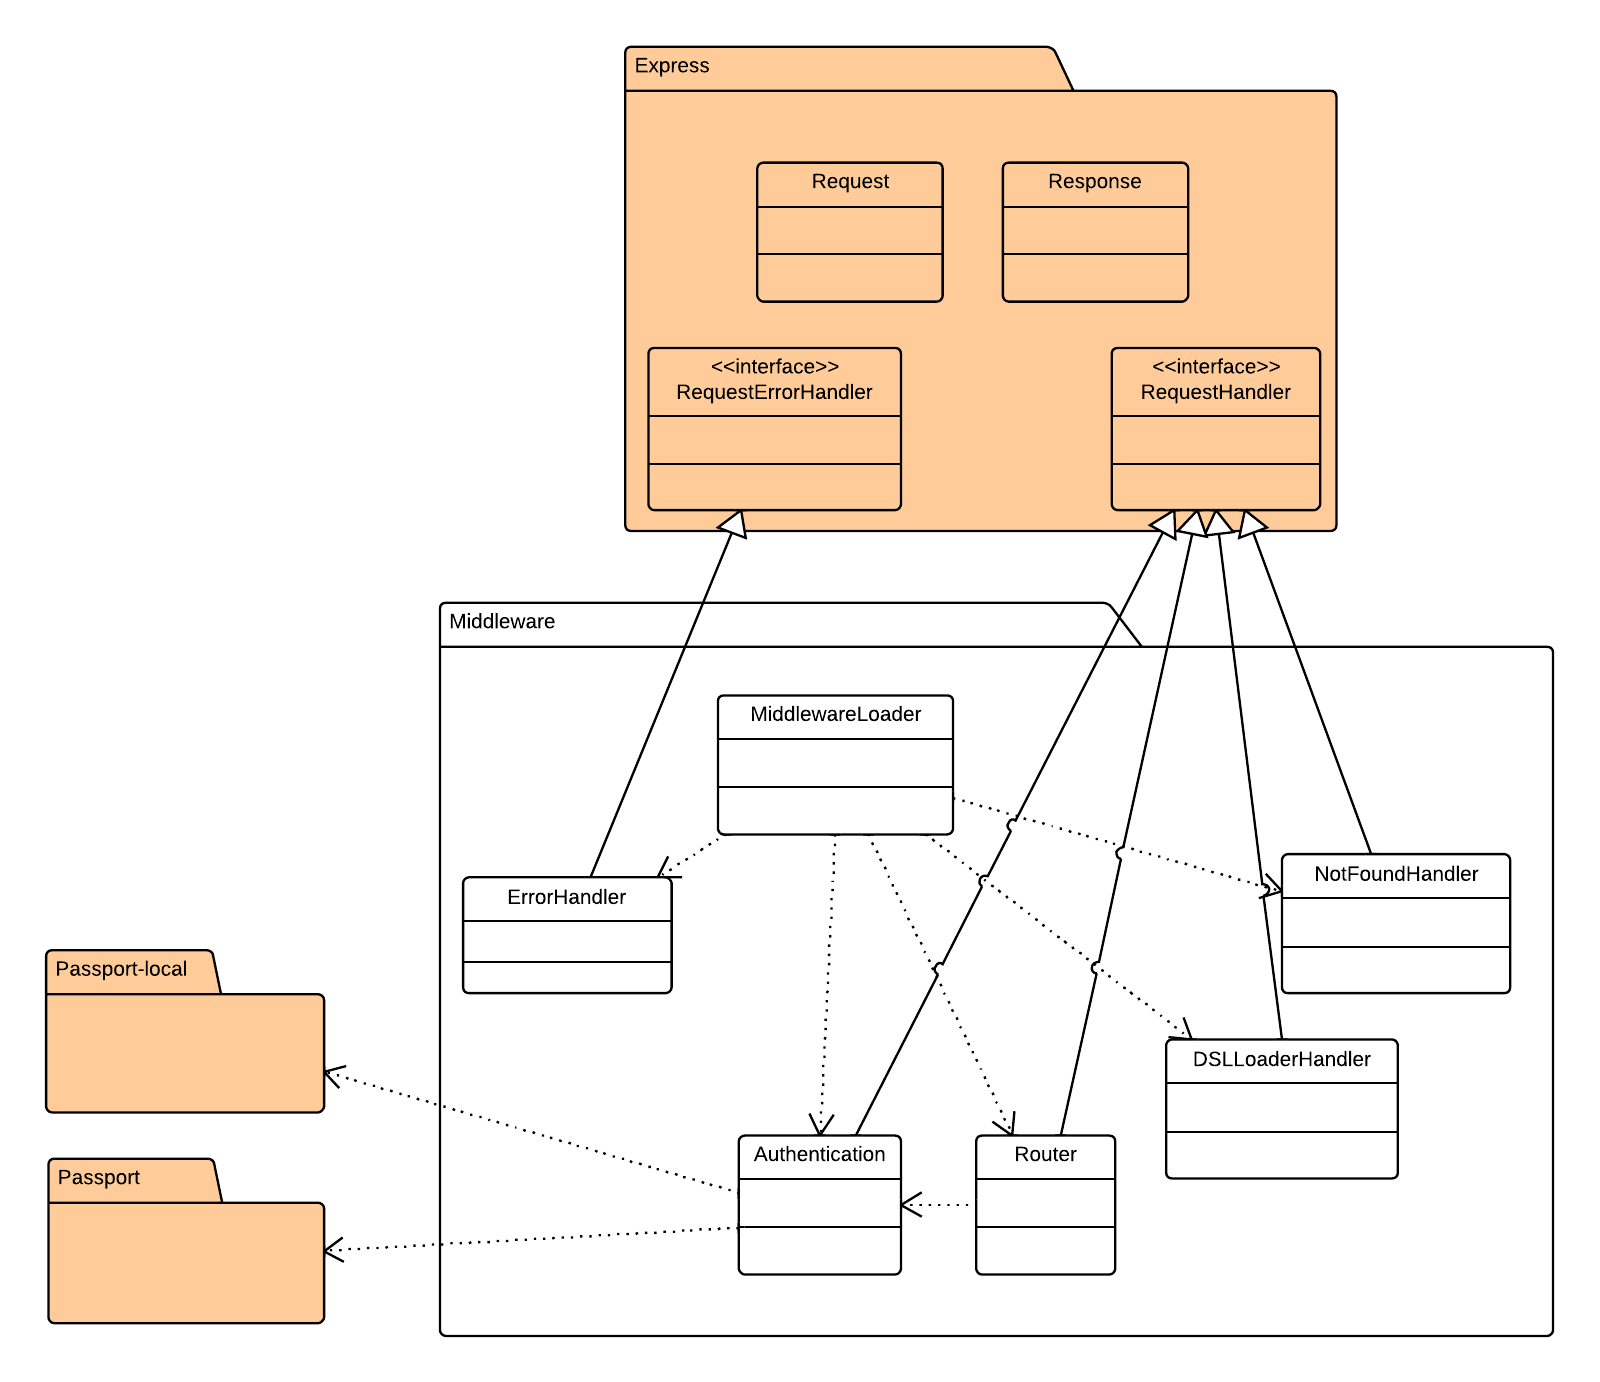
\includegraphics[width=\textwidth]{uml/package/Back-end::Lib::Controller::Middleware.png}  
        \caption{Componente Middleware}
      \end{center}  
    \end{figure} 
  \subparagraph{Descrizione} 
    \begin{itemize}
    \item[] \glossario{Package} contenente classi che costituiscono gli handler della catena di chiamate a cui viene
passata la responsabilità di gestire una richiesta, decorando quest’ultima con parametri e
metodi utilizzabili dai controller. Costituisce una parte controller nell’architettura \glossario{MVC}
del \glossario{Back-end} .

    \end{itemize} 
  \subsubsection{Controller}
  \paragraph{Informazioni sul package} 
    \begin{figure}[H] 
      \begin{center} 
        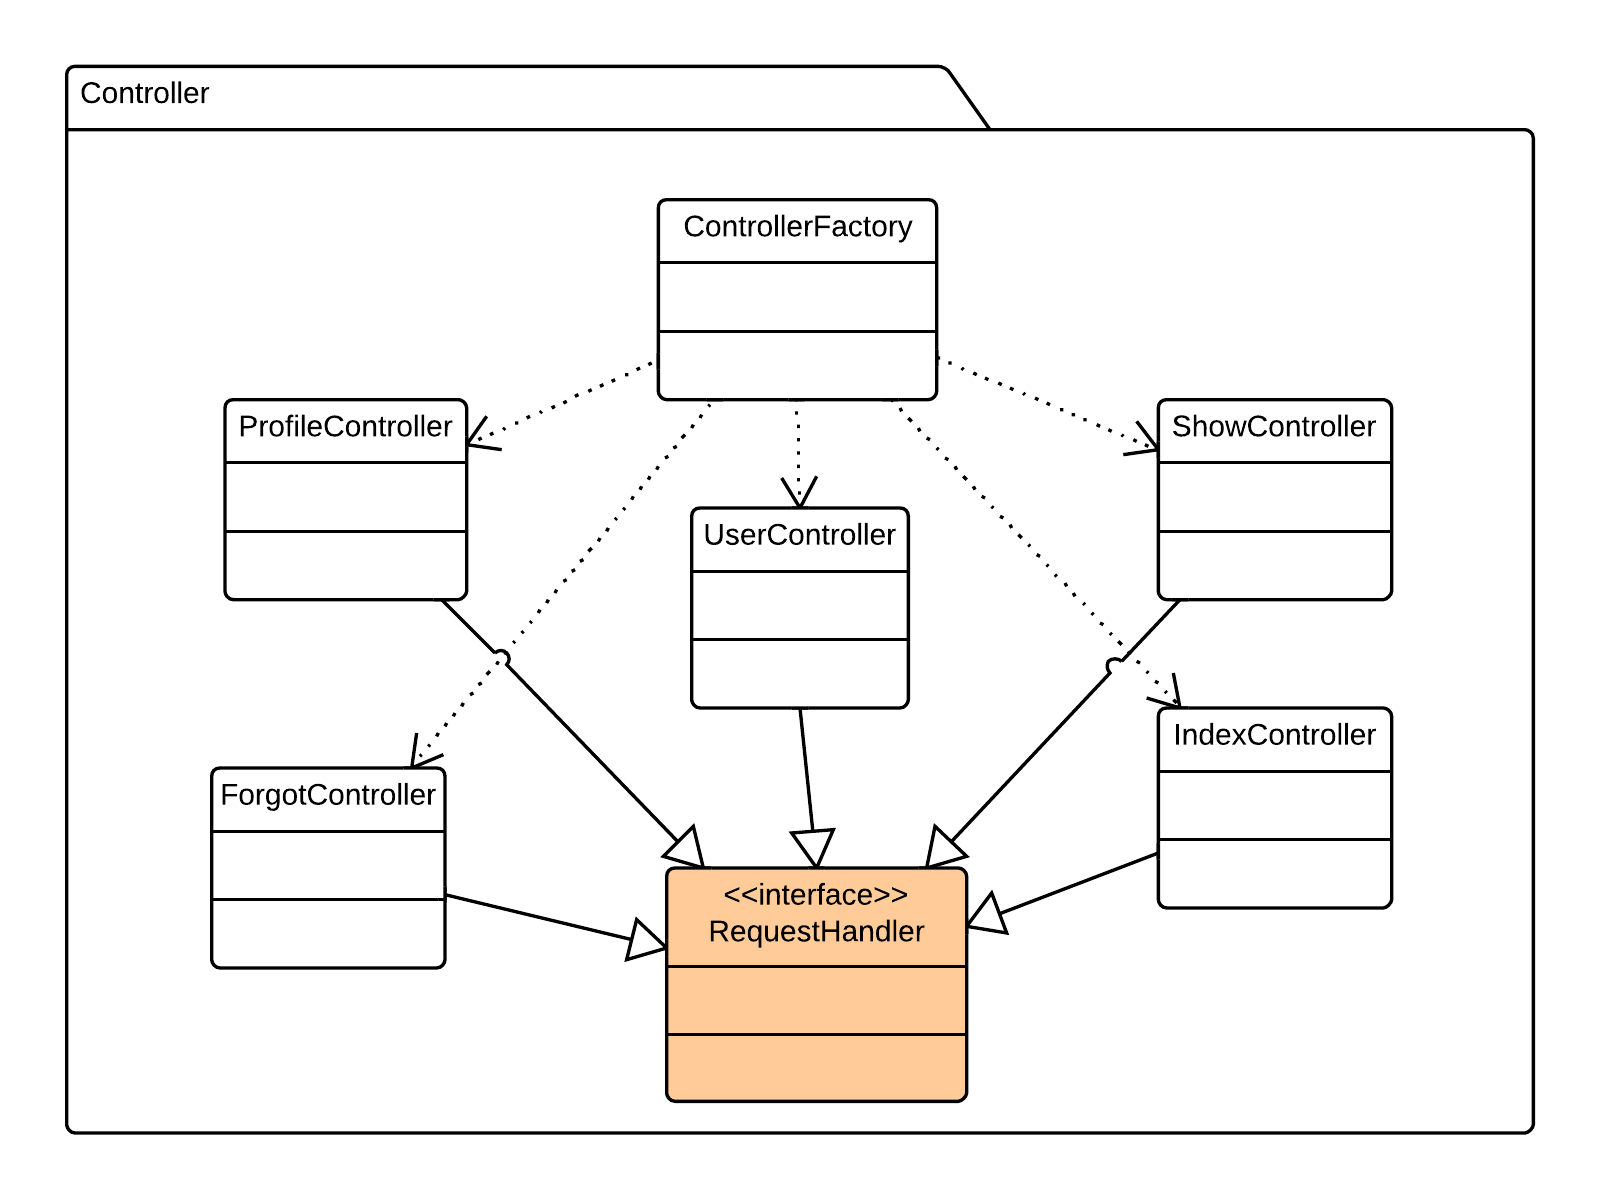
\includegraphics[width=\textwidth]{uml/package/Back-end::Lib::Controller::Controller.png}  
        \caption{Componente Controller}
      \end{center}  
    \end{figure} 
  \subparagraph{Descrizione} 
    \begin{itemize}
    \item[] \glossario{Package} per il componente che realizza parte controller nell’architettura mvc nel back-
end. Contiene classi per le funzionalità di controllo e visualizzazione delle risorse, dove ogni
classe gestisce in modo esclusivo una sola di queste, in base all’ \glossario{URI} .

    \end{itemize} 
  \subsubsection{Lib}
  \paragraph{Informazioni sul package} 
    \begin{figure}[H] 
      \begin{center} 
        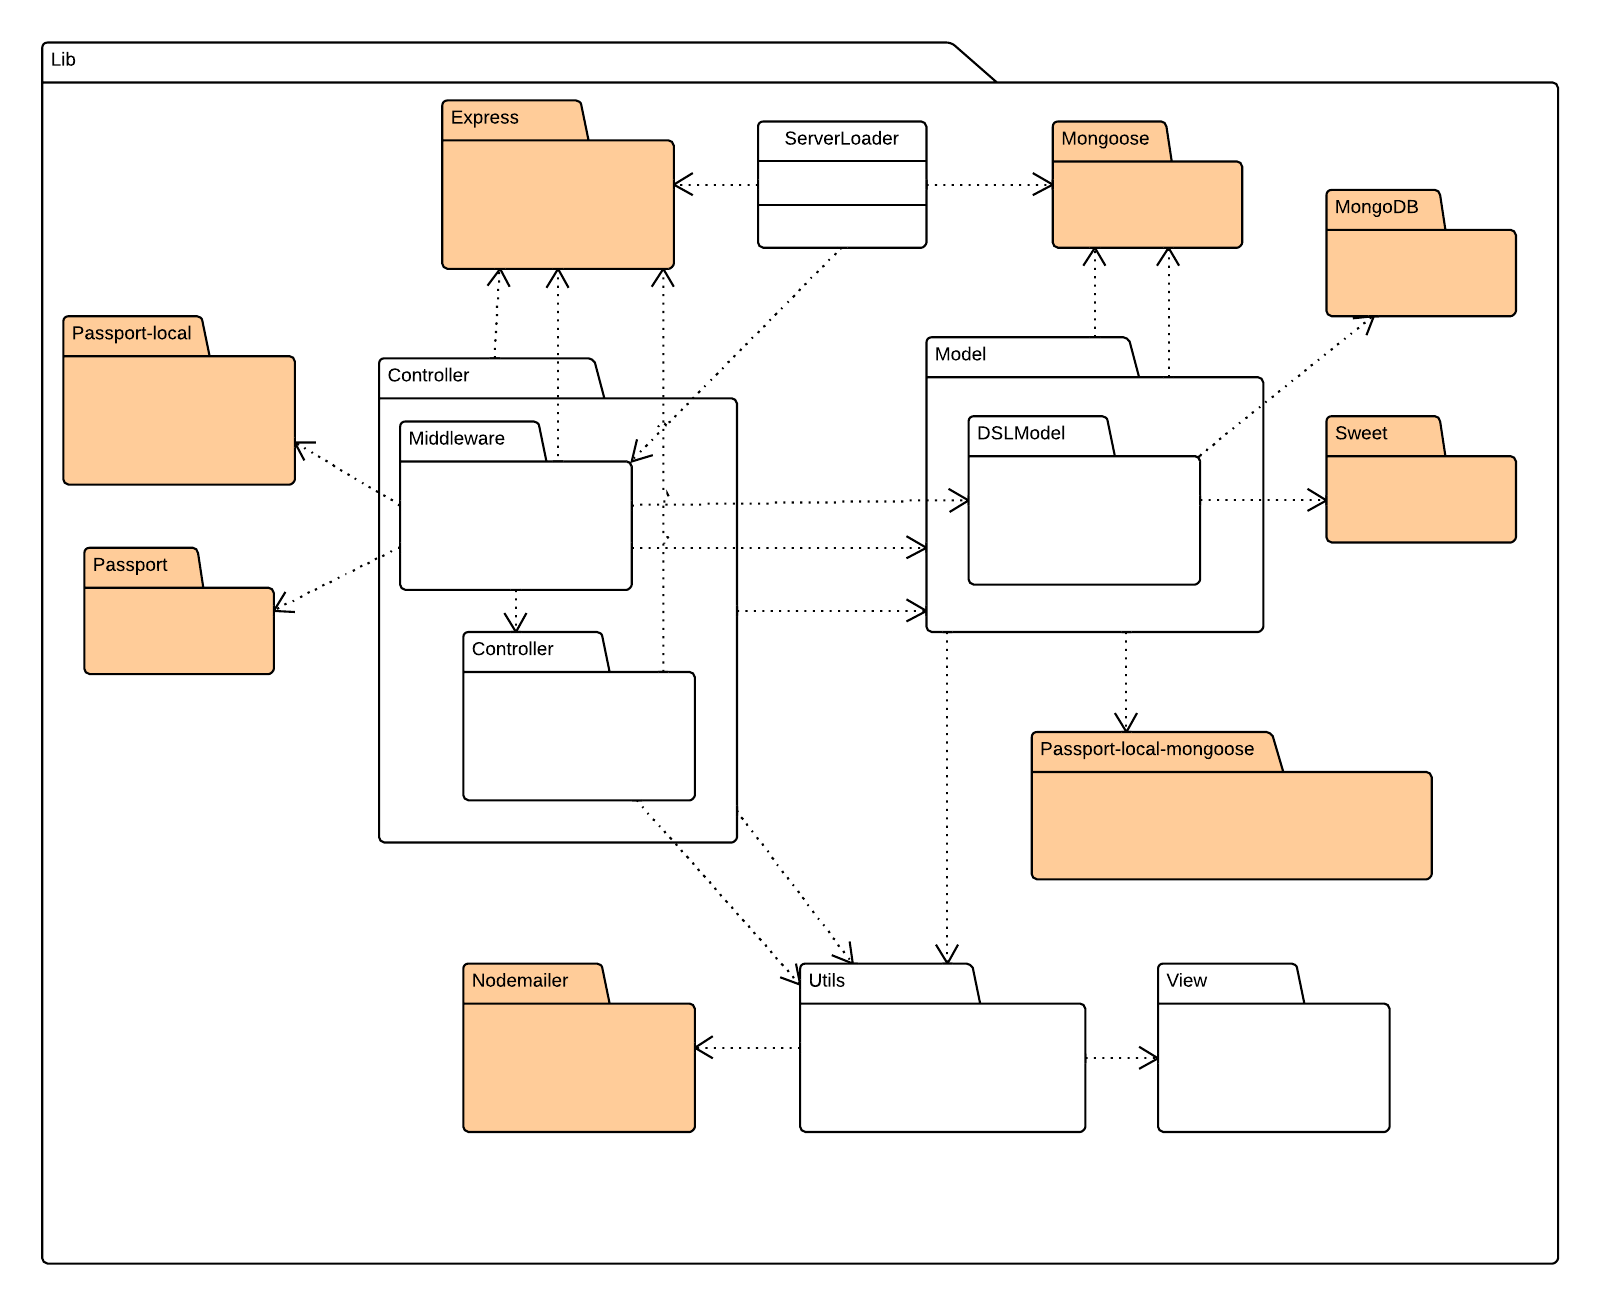
\includegraphics[width=\textwidth]{uml/package/Back-end::Lib.png}  
        \caption{Componente Back-end::Lib}
      \end{center}  
    \end{figure} 
  \subparagraph{Descrizione} 
    \begin{itemize}
    \item[] \glossario{Package} che costituisce la libreria principale dell’applicazione \glossario{MaaP}, che verrà fornita ai
developer per installare e utilizzare l’applicazione. Comprende gli script per l’installazione,
non rappresentati nei diagrammi in quanto non sono modellati come oggetti.

    \end{itemize} 
    \subparagraph{Package contenuti} 
    \begin{itemize}
        \item View
        \item Controller
        \item Model
    \end{itemize}
    \paragraph{Classi}
      \subparagraph{Back-end::Lib::Error}
        
        \textbf{\\ \\ Descrizione} 
          \begin{itemize}
            \item[] Classe che rappresenta un errore all'interno del package \texttt{Back-end::Lib}.
          \end{itemize}      
        \textbf{Utilizzo}  
          \begin{itemize}
            \item[] Viene utilizzata da tutte le classi presente all'interno del package \texttt{Back-end::Lib} per rappresentare un errore generato, identificandolo tramite nome, descrizione e codice.
          \end{itemize}